
\documentclass[preprint]{elsarticle}
%
\usepackage{url}
\usepackage{hyperref}
%\usepackage{caption}
%\usepackage{multirow}
%\usepackage{array}
%\usepackage{lscape}
%\usepackage{tikz}
%\usepackage{longtable}


\newcommand{\rem}[2]{{\bf [#1] #2}}

\begin{document}

\title{A Simple Survey on the Virtual Observatory}

\author[utfsm]{Mauricio Araya\corref{cor1}}

\ead{maray@inf.utfsm.cl}

\author[utfsm]{Mauricio Solar}

\ead{msolar@inf.utfsm.cl}

\author[utfsm]{Jonathan Antognini}

\ead{jantogni@alumnos.inf.utfsm.cl}

\address[utfsm]{Universidad T\'ecnica Federico Santa Mar\'ia\\
Avenida Espa\~na 1680, Valpara\'iso, Chile}

\begin{abstract}
%\boldmath
This paper presents a short survey on the astronomical Virtual Observatories (VOs) that are 
part of the International Virtual Observatory Alliance (IVOA). From how they are
distributed worldwide to their specialization range on the electromagnetic spectrum, 
we summarize key aspects of the current 21 VO members. Through the Registry
service, we explore the resources that the VO offer as a whole, and identify 
that even though the VO is already a mature initiative, there are important
challenges to address in the near future.
\end{abstract}

\maketitle




\section{Introduction}


\section{Distribution of IVOA Virtual Observatories Worlwide and its Projects}
\subsection{The IVOA}
From June 2002, projects of virtual observatories have come to integrate the
International Virtual Observatory Alliance (IVOA) under the \textbf{Guidelines
for Participation\footnote{The guidelines are available in a paper in PDF and
DOC format from
\url{http://www.ivoa.net/documents/latest/IVOAParticipation.html}}}. These were
founded through national and international governmental and private programs in
collaboration with various centers of scientific studies, universities and
others. Who integrate this project, the Virtual Observatory (VO), share
knowledge between them and the community in a standardized manner. They
themselves are who develop these standards for data exchange and
interoperability.\\

The table \ref{table:partners} shows the partners of IVOA to May 2013.\\

\begin{table}%[h!t]
\centering
\begin{tabular}{|p{7cm}|p{7cm}|}
	\hline
	\textbf{Project} & \textbf{URL} \\
	\hline
	Argentina Virtual Observatory & \url{http://nova.conicet.gov.ar/} \\
	\hline
	Armenian Virtual Observatory & \url{http://www.aras.am/Arvo/arvo.htm} \\
	\hline
	AstroGrid & \url{http://www.astrogrid.org/} \\
	\hline
	Australian Virtual Observatory & \url{http://aus-vo.org.au/} \\
	\hline
	Brazilian Virtual Observatory & \url{http://www.lna.br/bravo/} \\
	\hline
	Canadian Virtual Observatory &
    \url{http://www.cadc-ccda.hia-iha.nrc-cnrc.gc.ca/cvo/} \\
	\hline
    Chinese Virtual Observatory &
    \url{http://www.china-vo.org/} \\
	\hline
    European Space Agency &
    \url{http://www.sciops.esa.int/index.php?project=ESAVO} \\
	\hline
	European Virtual Observatory & \url{http://www.euro-vo.org/} \\
	\hline
	German Astrophysical Virtual Observatory & \url{http://www.g-vo.org/} \\
	\hline
	Hungarian Virtual Observatory & \url{http://hvo.elte.hu/en/} \\
	\hline
	Italian Virtual Observatory & \url{http://vobs.astro.it/} \\
	\hline
	Japanese Virtual Observatory & \url{http://jvo.nao.ac.jp/}\\
	\hline
	Observatorie Virtual France & \url{http://www.france-vo.org/} \\
	\hline
	Russian Virtual Observatory & \url{http://www.inasan.rssi.ru/eng/rvo/} \\
	\hline
	Spanish Virtual Observatory & \url{http://svo.cab.inta-csic.es/} \\
	\hline
	Ukranian Virtual Observatory & \url{http://www.ukr-vo.org/} \\
	\hline
	Virtual Astronomical Observatory & \url{http://www.usvao.org/} \\
	\hline
	Virtual Observatory India & \url{http://vo.iucaa.ernet.in/~voi/} \\
	\hline
\end{tabular}
\caption{IVOA Partners.}
\label{table:partners}
\end{table}

Almost half of IVOA virtual observatories are supported in Europe: 9 of the
total; 1 belong to Oceania, 4 to America and 5 to Asia\footnote{As the mayor
part of Rusia's territory is in Asia, it will be considered like a virtual
observatory of Asian continent.}. The figure 1 shows the distribution of the
IVOA's membership per continent.\\

\begin{figure}%[h]
\begin{center}
	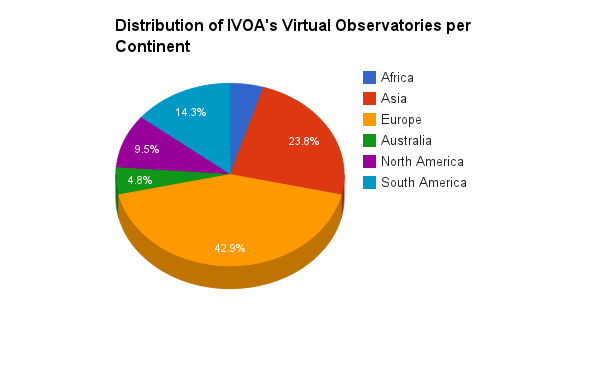
\includegraphics[width=110mm]{img/vo_distribution.png}
	\caption{International Virtual Observatory Alliance distribution per
             continent.}
\end{center}
\end{figure}

If Chile became part of International Virtual Observatory Alliance, the
distribution of the members per continent will be as shown in the figure 2.\\

\begin{figure}%[h]
\begin{center}
	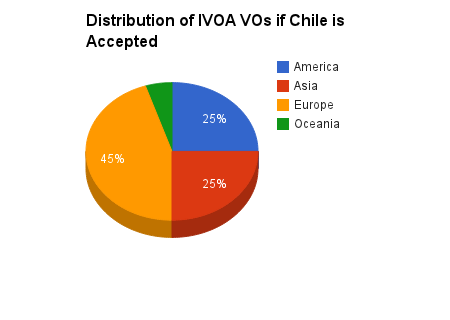
\includegraphics[width=110mm]{img/if_chile.png}
	\caption{International Virtual Observatory Alliance distribution per
             continent if Chile is accepted.}
\end{center}
\end{figure}

Without considering the status of the internal projects of the virtual
observatories, the membership of Chile would contribute to the cooperation,
development and interoperability from America in the same percent that Asia.
Furthermore, this fact would be very significant, because a large numbers of
astronomical centers like observatories are placed in this country.  For now, is
intended to work with a certain quantity of data of ALMA.\\


\subsection{Summary of Tools and Projects}

The standards and services of a VO are meant to be used in the end 
by applications. The Applications working group have defined only two major
standards for application interoperability beyond the services standards: 
(1) the Simple Application Messaging Protocol (SAMP), and (2) the VOTable
format. These standards, plus all the other protocols and standards 
allows VO-compliant tools to be developed, which are the endpoints for
science production. In the next table we summarize the most used tools
and they status.

%%%%%%%%%%%%%%%%%%%%%%%%%%%%%%%%%%%%%%%%%%%%%%%%%%%%%%%%%%%%%%%%%%%%%%%%%%%%%%%%%
%%%%%%%%%%%%%%%%%%%%%%%%%%%%%%%%%$Data Access%%%%%%%%%%%%%%%%%%%%%%%%%%%%%%%%%%%%
%%%%%%%%%%%%%%%%%%%%%%%%%%%%%%%%%%%%%%%%%%%%%%%%%%%%%%%%%%%%%%%%%%%%%%%%%%%%%%%%%
\begin{table*}[h]
	\centering
	\begin{tabular}{|l|l|p{8.5cm}|}
	\hline
	\textbf{User Tool} & \textbf{Country} &  \textbf{Comment}\\
	\hline
  Cross-Comparision Tool & USA & a web tool that performs croos-comparisons between one table supplied by the user and other of an online source 
								catalog, for a user-specified match radius. This returns the all sources in the online catalog that are within the radius.\\
	\hline								 
  Data Discovery Tool & USA &  A web tool that allows to find datasets from astronomical collections known to the VO like the Hubble Space Telescope 
									(HST), the Chandra X-ray Observatory, the Spitzer Space Telescope, among other.\\
	\hline								 
  Time Series Search Tool & USA & A web tool that allows to access the time series data sets at the Harvard Time Series Center (TSC), the NASA 
									Exoplanet Archive and the Catalina Real-Time Transient Survey, and analize them with the periodogram application 
									of the NASA Exoplanet Archive.\\
  \hline
  Iris & USA & A downloadable application for the finding, plotting and fitting the 
			Spectral Energies Distributions (SEDs). \\
	\hline								 
  Seleste & USA & \\
	\hline								 
  Skyview & USA & \\
	\hline								 
  Specview & USA & \\
  \hline
  WCSFIXER & USA & \\
  \hline 
  Montage & USA & \\
  \hline
  Xamin & USA & \\
	\hline								 
  Aladin & France & Widely-used VO tool that allows searching, visualizing
and perform basic operation to images, spectra and catalogs.\\
	\hline								 
  Cassis & France & \\
	\hline								 
  Cross-Match Service & France  & \\
	\hline								 
  AppLauncher & France & \\
	\hline								 
  X-Match & France & \\
	\hline								 
   VOSA & Spain & \\
	\hline								 
  VOSED & Spain & \\
	\hline								 
  TESELA & Spain &  a service that allows to access the catalog of blank
regions. It is based on the application of the Delaunay triangulation\\
	\hline								 
  Filter Profiles & Spain & \\
   \hline
	VODesktop & UK & an analysis tools wich allows limit the choice of resources through specific data saving.\\
	\hline								 
  Topcat & UK &  An interactive graphical viewer and editor for tabular data for
formats like the Flexible Image Transport System (FITS) \\
	\hline								 
	\hline								 
  Splat & Germany & \\
	\hline								 
   VOSpec & Europe & A multi-wavelength spectral analysis tool with access to
atomic and \\
	\hline								 
 AstroStat & India & a software tool that allows astronomers to use both and sophisticated statical routines on large datasets uploaded in VOTable or
									ASCII format. \\
	\hline								 
  Visivo & Italy & \\
	\hline								 
	Skynode & Italy & A web service that allows to query in the VVDS catalogs. \\
	\hline		
	\end{tabular}
	\caption{Data Access}
	\label{table:da}
\end{table*}



\section{VO Services}
%%%%%%%%%%%%%%%%%%%%%%%%%%%%%%%%%%%%%%%%%%%%%%%%%%%%%%%%%%%%%%%%%%%%%%%%%%%%%%%%%
%%%%%%%%%%%%%%%%%%%%%%%%%%%%%%%%%$Data Access%%%%%%%%%%%%%%%%%%%%%%%%%%%%%%%%%%%%
%%%%%%%%%%%%%%%%%%%%%%%%%%%%%%%%%%%%%%%%%%%%%%%%%%%%%%%%%%%%%%%%%%%%%%%%%%%%%%%%%
\subsection{Data Access}
\begin{table*}[h!t]
	\centering
	\begin{tabular}{|l|l|p{12.5cm}|}
	\hline
	CVO 	& Data Sharing (VOSpace 2.0) &  A service that allows to share files and collaborate with team members \\
			& Table Access Protocol (TAP-1.0) &	A model that implements a standard view for \textbf{Table Access Protocol (TAP-1.0)}. \\
			& Observation Model Core Components & A model that implements a standard view for \textbf{Table Access Protocol (TAP-1.0)}. \\
			& Simple Image Access (SIA-1.0) & a SIA-1.0 compliant query service for easy access to calibrated images from most our data collections. \\
	\hline
	VAO		& Data Discovery Tool & A web tool that allows to find datasets from astronomical collections known to the VO like the Hubble Space Telescope 
									(HST), the Chandra X-ray Observatory, the Spitzer Space Telescope, among other.\\
			& Time Series Search Tool & A web tool that allows to access the time series data sets at the Harvard Time Series Center (TSC), the NASA 
									Exoplanet Archive and the Catalina Real-Time Transient Survey, and analize them with the periodogram application 
									of the NASA Exoplanet Archive.\\
	\hline
	BRAVO	& BRAVO@LNA & Making of a virtual observatory dedicated to Southern Astrophysical Research Telescope (SOAR) data from Brazilian astronomers.  \\
	\hline
	ChiVO	& Conceptual Design of a VO for ALMA & A degree thesis that through the researching and analysis of query 
									languages, formats and the semantic of OVA (in its Spanish acronym), and the definition of it intends to make a 
									conceptual design for the ALMA observatory.\\
	\hline								
	HVO		& Spectrum Service for VO & A proposal that intends to add several features and make two substantial improvements to the web services that 
									contains spectra of galaxies and the other astronomical objects.\\
			& Synthetic Spectrum Service & A proposal that intends to serve, as a web service, the ready made spectra for the users.\\
			& Debrecen Photoheliographic Data & A sunspot catalogue with the heliographic positions and the areas of sunspots. A continuation of Greenwich 
									Photoheliographic Results (GPR) that had been discontinued on 1976.\\
	\hline								
	AstroGrid& Topcat & An interactive graphical viewer and editor for tabular data for formats like the Flexible Image Transport System (FITS) 
									and VOTable. \\
			& VODesktop & an analysis tools wich allows limit the choice of resources through specific data saving.\\
	\hline		
	ESA-VO	& DALToolKit & A downloadable software based on JAVA that allows to publish in the VO following the Data Access Layer (DAL) protocol. It 
									converts incoming standard DAL requests into database specific SQL queires, then serializes the database result into VOTable 
									responses. \\
			& IVOA Resource Registry & the official EURO-VO resource registry under the name of EURO-VO Full Harvestable VO Resource Registry that \\
			& VOSpec & A multi-wavelength spectral analysis tool with access to atomic and molecular databases, spectra and theorical models registered 
									in the VO. It can be downloadable and accessed through Internet.\\
	\hline								
	GAVO	& GAVO Data Center & A growing collection of data and services provided on behalf of third parties. Some of the GAVO services are also 
									available on \url{http://dc.zah.uni-heidelberg.de/}\\
			& MPA Simulations access & A web service for querying the results of the Millennium simulation using SQL.\\
			& MultiDark Database & A service wich gives access to data from MultiDark and Bolshoi simulations using SQL queries.  It based on the Millennium 
									Web Application. \\
			& RAVE archive search & An access to a growing archive of radial velocities for more than 400 000 stars.\\
			& TheoSSA & A service for providing spectral energy distributions based on model atmosphere calculations.\\
	\hline		
	SVO		& TESELA & a service that allows to access the catalog of blank regions. It is based on the application of the Delaunay triangulation
									 of the sky. \\
	\hline								 
	VObs.it	& SIAP & A web services that provides the public Hubble Space Telescope/Advanced Camera for Surveys (HST/ACS) Great Observatories Origins 
									Deep Survey (GOOD) data within the VIMOS\footnote{VIMOS is a \textbf{VI}sible imaging \textbf{M}ulti-\textbf{O}bject 
									\textbf{S}pectrograph, a spectrograph for the European Southern Observatory Very Large Telescope array (ESO-VLT).}-VLT
									Deep Survey-Chandra Deep Field South (VVDS-CDFS).\\
			& SSAP & A web service that allows to access the VVDS-F02-DEEP spectra. \\
			& Cone Search & A web service that allows to query in the VVDS-CDFS catalog.  \\
			& Skynode & A web service that allows to query in the VVDS catalogs. \\
	\hline		
	China-VO& FITS Manager & A downloadable application, as a collaboration project between China-V0 and VOI, to manage FITS, VOTable, among other files, 
								hosted in personal computers \footnote{FITS Manager (FM) is downloadble from \url{http://fm.china-vo.org/app/fm.zip}.}  \\
			& VO Data Access Service & A data access framework that allows to query large volumes of astronomical resources like catalogs, spectrum 
									and images through the command line, a graphical interface or webpage.\\
			& FITS Header Archiving System & A downloadable tool that allows to view and import the FITS header files into a database table for single or 
									multiple files. It was also developed by the IBM Center, Tianjin University (TU) and e-Science application research 
									center, Computer Network Information Center (CNIC), Chinese Academy of Sciences (CAS).\\
			& Imaging Processing and analysis tool & a downloadable imaging processing and analysis tool developed in JAVA that allows to visualize sky 
									images and access related data from the Beijing Astronomical Data Center (BADC). \\
			& VOTable2XHTML & A XSLT stylesheet that can be used to transform VOTable file into XHTML file.\\
			& SkyMouse & A search engine that allows to access astronomical services like web service and CGI service. \\
	\hline		
	JVO		& JVO portal service & A site as portal to various kind of astronomical resources from the Subaru Telescope, Sloan Digital Sky and ALMA, among 
									other. \\
	\hline								
	VOI		& VOIPortal & An entry to all VOI web services. Can be browse the data downloading or through VOIMosaic and PyMorph web applications.\\
			& Mosaic Service & A software that allows to make mosaic, with SWarp\footnote{The SWarp tool is available from \url{http://www.astromatic.
									net/software/swarp}} and SExtractor\footnote{The SExtractor tool is available from \url{http://www.astromatic.
									net/software/sextractor}} and STIFF, of images retrieved from SDSS\footnote{The SDSS image server is available from 
									\url{http://casjobs.sdss.org/vo/DR7SIAP/SIAP.asmx}}, 2MASS\footnote{The 2MASS image server is available from 
									\url{http://irsa.ipac.caltech.edu/applications/2MASS/IM/}} and HST\footnote{The HST image server is available from 
									\url{http://archive.stsci.edu/siap/search.php}} image servers.\\
			& PyMorph Service & A software that allows to derive morphological parameters for galaxy images. Is possible to provide to it the output FITS
									files generated by Mosaic Service.\\
			& VOPlot & A software tool developed in JAVA that allows to visualize astronomical data available in VOTable, ASCII and FITS formats.\\
			& VOMegaPlot & a software tool developed in JAVA that allows to visualize astronomical data available in VOTable format. It looks just like 
									VOPlot. There is a client-server version.\\
			& AstroStat & a software tool that allows astronomers to use both and sophisticated statical routines on large datasets uploaded in VOTable or
									ASCII format. \\
			& VOCat & a software tool that converts astronomical catalogs to MySQL databases. \\
			& VOPlatform& a software tool developed in JAVA that allows to place their frequently used VO tools and datasets with others resourcers like 
									documents, links, among other. \\
			& VOConvert & A software tool that converts ASCII to VOTable files, FITS to VOTable and VOTable to ASCII. \\
			& Android Cosmological Calculator & an Android aplication that allows to input the Hubble constant, $ \Omega_{m} $(matter), $ \Omega_{\lambda} 
									$ (vacuum) and the redshift($ z $), and returns the current age of the Universe, the co-moving radial distance and 
									volume and the angular size distance at the specified redshift, and the luminosity distance.\\
			& Android Name Resolver & An Android application that allows to input the name of celestial object and returns information of this like 
									RA/DEC values, redshift, proper motion, parallax, among other.\\
			& CSharpFITS Package & A C\# .NET port of Tom McGlynn's nom.tam.fits JAVA packages\footnote{The C\# .NET port of Tom McGlynn's nom.tam.fits 
									JAVA packages are availablre from \url{http://heasarc.gsfc.nasa.gov/docs/heasarc/fits/java/v0.9/javadoc/}}.\\
			& VOTable JAVA Streaming Writer & A software that converts data streams in non-VOTable format, like ASCII or FITS, to the VOTable format. \\
			& C++ parser for VOTable & A C++ library to access VOTable files. It has a non-streaming and streaming version.\\
			& Fits Manager & A web-based tool for viewing, creating, adding extensions and converting FITS files.\\
			& HCT Data Archive System & a web-based system that archives the observational data generated by the Himalayan Chandra Telescope (HCT), a 2 [m]
									 aperture optical-infrared telescope manufactured by the EOS Technologies Inc. and remotely operated via dedicated
									 satellite link.\\
	\hline
	\end{tabular}
	\caption{Data Access}
	\label{table:integrantes}
\end{table*}


\begin{itemize}
%\item \textbf{CVO}
%\item \textbf{Data Sharing (VOSpace 2.0)}:
%a service that allows to share files and collaborate with team members.

%\item \textbf{Table Access Protocol (TAP-1.0)}:
%a service that allows the access to all the data
%described by the Common Archive Observation Model (CAOM) in use at the CADC and
%tables from other projects.

%\item \textbf{Observation Model Core Components (ObsCore-1.0)}:
%a model that implements a standard view for \textbf{Table Access Protocol (TAP-1.0)}.

%\item \textbf{Simple Image Access (SIA-1.0)}:
%a SIA-1.0 compliant query service for easy access to calibrated images from most
%our data collections.

%\item \textbf{VAO}
%\item \textbf{Data Discovery Tool}:
%a web tool that allows to find datasets from astronomical collections known to
%the VO like the Hubble Space Telescope (HST), the Chandra X-ray Observatory, the
%Spitzer Space Telescope, among other.

%\item \textbf{Time Series Search Tool}:
%a web tool that allows to access the time series data sets at the Harvard Time
%Series Center (TSC), the NASA Exoplanet Archive and the Catalina Real-Time
%Transient Survey, and analize them with the periodogram application of the NASA
%Exoplanet Archive.

%\item \textbf{BRAVO}
%\item \textbf{BRAVO@LNA}:
%making of a virtual observatory dedicated to Southern Astrophysical Research
%Telescope (SOAR) data from Brazilian astronomers.  

%\item \textbf{ChiVO}
%\item \textbf{Conceptual Design of a Virtual Astronomical Observatory for ALMA}:
%a degree thesis that through the researching and analysis of query languages,
%formats and the semantic of OVA (in its Spanish acronym), and the definition of
%it intends to make a conceptual design for the ALMA observatory.

%\item \textbf{HVO}
%\item \textbf{Spectrum Service for VO}:
%a proposal that intends to add several features and make two substantial
%improvements\footnote{Does not specified what several features and the two
%substantial improvements.} to the web services that contains spectra of galaxies
%and the other astronomical objects.

%\item \textbf{Synthetic Spectrum Service}:
%a proposal that intends to serve, as a web service, the ready made spectra for
%the users.

%\item \textbf{Debrecen Photoheliographic Data (DPD)}:
%a sunspot catalogue with the heliographic positions and the areas of sunspots. A
%continuation of Greenwich Photoheliographic Results (GPR) that had been
%discontinued on 1976.

%\item \textbf{AstroGrid}
%\item \textbf{Topcat}:
%an interactive graphical viewer and editor for tabular data for formats like the
%Flexible Image Transport System (FITS) and VOTable.

%\item \textbf{VODesktop}:
%an analysis tools wich allows limit the choice of resources through specific
%data saving.

%\item \textbf{ESA-VO}
%\item \textbf{DALToolKit}:
%a downloadable software based on JAVA that allows to publish in the VO following
%the Data Access Layer (DAL) protocol. It converts incoming standard DAL requests
%into database specific SQL queires, then serializes the database result into
%VOTable responses. 

%\item \textbf{IVOA Resource Registry}:
%the official EURO-VO resource registry under the name of EURO-VO Full
%Harvestable VO Resource Registry that 

%\item \textbf{VOSpec}:
%a multi-wavelength spectral analysis tool with access to atomic and molecular
%databases, spectra and theorical models registered in the VO. It can be
%downloadable and accessed through Internet.

%\item \textbf{GAVO}
%\item \textbf{GAVO Data Center}:
%a growing collection of data and services provided on behalf of third parties.
%Some of the GAVO services are also available on
%\url{http://dc.zah.uni-heidelberg.de/}

%\item \textbf{MPA Simulations access}:
%a web service for querying the results of the Millennium simulation using SQL.

%\item \textbf{MultiDark Database}:
%a service wich gives access to data from MultiDark and Bolshoi simulations using
%SQL queries.  It based on the Millennium Web Application.

%\item \textbf{RAVE archive search}:
%an access to a growing archive of radial velocities for more than 400 000 stars.

%\item \textbf{TheoSSA}:
%a service for providing spectral energy distributions based on model atmosphere
%calculations.

%\item \textbf{SVO}
%\item \textbf{TESELA}:
%a service that allows to access the catalog of blank regions. It is based on the
%application of the Delaunay triangulation of the sky.

%\item \textbf{VObs.it}
%\item \textbf{SIAP}:
%a web services that provides the public Hubble Space Telescope/Advanced Camera
%for Surveys (HST/ACS) Great Observatories Origins Deep Survey (GOOD) data within
%the VIMOS\footnote{VIMOS is a \textbf{VI}sible imaging
%\textbf{M}ulti-\textbf{O}bject \textbf{S}pectrograph, a spectrograph for the
%European Southern Observatory Very Large Telescope array (ESO-VLT).}-VLT Deep
%Survey-Chandra Deep Field South (VVDS-CDFS).

%\item \textbf{SSAP}:
%a web service that allows to access the VVDS-F02-DEEP spectra.

%\item \textbf{CONE SEARCH}:
%a web service that allows to query in the VVDS-CDFS catalog. 

%\item \textbf{SKYNODE}:
%a web service that allows to query in the VVDS catalogs. 

%\item \textbf{China-VO}
%\item \textbf{FITS Manager (FM)}:
%a downloadable application, as a collaboration project between China-V0 and VOI,
%to manage FITS, VOTable, among other files, hosted in personal computers
%\footnote{FITS Manager (FM) is downloadble from
%\url{http://fm.china-vo.org/app/fm.zip}.} 

%\item \textbf{VO Data Access Service (VO-DAS)}:
%a data access framework that allows to query large volumes of astronomical
%resources like catalogs, spectrum and images through the command line, a
%graphical interface or webpage.

%\item \textbf{FITS Header Archiving System (FitHAS)}:
%a downloadable tool that allows to view and import the FITS header files into a
%database table for single or multiple files. It was also developed by the IBM
%Center, Tianjin University (TU) and e-Science application research center,
%Computer Network Information Center (CNIC), Chinese Academy of Sciences (CAS).

%\item \textbf{Imaging Processing and analysis tool for China\_VO (VO\_IMPAT)}:
%a downloadable imaging processing and analysis tool developed in JAVA that
%allows to visualize sky images and access related data from the Beijing
%Astronomical Data Center (BADC). 

%\item \textbf{VOTable2XHTML}
%a XSLT stylesheet that can be used to transform VOTable file into XHTML file.

%\item \textbf{SkyMouse}:
%a search engine that allows to access astronomical services like web service and
%CGI service.

%\item \textbf{JVO}
%\item \textbf{JVO portal service}:
%a site as portal to various kind of astronomical resources from the Subaru
%Telescope, Sloan Digital Sky and ALMA, among other.

%\item \textbf{VOI}
%\item \textbf{VOIPortal}:
%an entry to all VOI web services. Can be browse the data downloading or through
%VOIMosaic and PyMorph web applications.

%\item \textbf{Mosaic Service}:
%a software that allows to make mosaic, with SWarp\footnote{The SWarp tool is
%available from \url{http://www.astromatic.net/software/swarp}} and
%SExtractor\footnote{The SExtractor tool is available from
%\url{http://www.astromatic.net/software/sextractor}} and STIFF, of images
%retrieved from SDSS\footnote{The SDSS image server is available from
%\url{http://casjobs.sdss.org/vo/DR7SIAP/SIAP.asmx}}, 2MASS\footnote{The 2MASS
%image server is available from
%\url{http://irsa.ipac.caltech.edu/applications/2MASS/IM/}} and HST\footnote{The
%HST image server is available from
%\url{http://archive.stsci.edu/siap/search.php}} image servers.

%\item \textbf{PyMorph Service}:
%a software that allows to derive morphological parameters for galaxy images. Is
%possible to provide to it the output FITS files generated by Mosaic Service.

%\item \textbf{VOPlot}:
%a software tool developed in JAVA that allows to visualize astronomical data
%available in VOTable, ASCII and FITS formats.

%\item \textbf{VOMegaPlot}:
%a software tool developed in JAVA that allows to visualize astronomical data
%available in VOTable format. It looks just like VOPlot. There is a client-server
%version.

%\item \textbf{AstroStat}:
%a software tool that allows astronomers to use both and sophisticated statical
%routines on large datasets uploaded in VOTable or ASCII format.

%\item \textbf{VOCat}:
%a software tool that converts astronomical catalogs to MySQL databases. 

%\item \textbf{VOPlatform}:
%a software tool developed in JAVA that allows to place their frequently used VO
%tools and datasets with others resourcers like documents, links, among other.

%\item \textbf{VOConvert (ConVOT)}:
%a software tool that converts ASCII to VOTable files, FITS to VOTable and
%VOTable to ASCII.

%\item \textbf{Android Cosmological Calculator}:
%an Android aplication that allows to input the Hubble constant, $ \Omega_{m} $
%(matter), $ \Omega_{\lambda} $ (vacuum) and the redshift($ z $), and returns the
%current age of the Universe, the co-moving radial distance and volume and the
%angular size distance at the specified redshift, and the luminosity distance.

%\item \textbf{Android Name Resolver}:
%an Android application that allows to input the name of celestial object and
%returns information of this like RA/DEC values, redshift, proper motion,
%parallax, among other.

%\item \textbf{CSharpFITS Package}:
%a C\# .NET port of Tom McGlynn's nom.tam.fits JAVA packages\footnote{The C\#
%.NET port of Tom McGlynn's nom.tam.fits JAVA packages are availablre from
%\url{http://heasarc.gsfc.nasa.gov/docs/heasarc/fits/java/v0.9/javadoc/}}.

%\item \textbf{VOTable JAVA Streaming Writer}:
%a software that converts data streams in non-VOTable format, like ASCII or FITS,
%to the VOTable format.

%\item \textbf{C++ parser for VOTable}:
%a C++ library to access VOTable files. It has a non-streaming and streaming
%version.

%\item \textbf{Fits Manager}:
%a web-based tool for viewing, creating, adding extensions and converting FITS
%files.

\item \textbf{HCT Data Archive System}:
a web-based system that archives the observational data generated by the
Himalayan Chandra Telescope (HCT), a 2 [m] aperture optical-infrared telescope
manufactured by the EOS Technologies Inc. and remotely operated via dedicated
satellite link.

\end{itemize}

%%%%%%%%%%%%%%%%%%%%%%%%%%%%%%%%%%%%%%%%%%%%%%%%%%%%%%%%%%%%%%%%%%%%%%%%%%%%%%%%%
%%%%%%%%%%%%%%%%%%%%%%%%%%%%%%%Grid and Cloud%%%%%%%%%%%%%%%%%%%%%%%%%%%%%%%%%%%%
%%%%%%%%%%%%%%%%%%%%%%%%%%%%%%%%%%%%%%%%%%%%%%%%%%%%%%%%%%%%%%%%%%%%%%%%%%%%%%%%%

\subsection{Grid and Cloud}
\begin{itemize}
\item \textbf{VAO}
\item \textbf{Cross-Comparision Tool}:
a web tool that performs croos-comparisons between one table supplied by the
user and other of an online source catalog, for a user-specified match radius.
This returns the all sources in the online catalog that are within the radius.

\item \textbf{BRAVO}
\item \textbf{BRAVO@INPE}:
generate investment in information technology on Computational Infraestructure,
Data Grid, Data Processing and Data Mining.

\item \textbf{ChiVO}
\item \textbf{Automatic Astronomical Different Scales Structures Detection and
Classification within Astronomical Images}:
a magister thesis that intends to make a software tool that finds directly
astronomical objects within astronomical images through the wavelet mathematical
tool and a machine learning system.

\item \textbf{Indexing of Astronomical Objects}:
a degree thesis that intends to design and implement an software tool that allow
make an R-tree index of FITS astronomical images based on their celestial
coordinates.

\item \textbf{HVO}
\item \textbf{Photometric Redshift Estimation}:
a proposal that intends to execute as a web service a method developed by
themselves that is capable to estimate redshift from photometry increasing by
two orders of magnitude the objects number of known distance. 

\item \textbf{Linking WebServices to GRID clusters}:
a proposal that intends, among other, to improvement the operating systems inter
communication, because there are simulations optimized for differents SOs and
the rewritten of the codes for one different in some cases results a
inaccessible task.

\item \textbf{Information Bulletin on Variable Stars}:
a bulletin on benhalf of the Commission 27\footnote{International Astronomical
Union. (2005, November). Commission 27. Variable Stars (Etoiles Variables).
Retrieved from \url{http://www.konkoly.hu/IAUC27/}} and
42\footnote{International Astronomical Union. (2014). Comision 42: Close Binary
Stars. Retrieved from: \url{http://www.konkoly.hu/IAUC42/}} of the International
Astronomical Union (IAU), published by the Konkoly Observatory of the Hungarian
Academy of Sciences. 

\item \textbf{AstroGrid}
\item \textbf{AstroRuntime}:
an API implemented in JAVA wich facilitates the access to the \textbf{VODesktop}
services from almost any programming language \footnote{On the AstroGrid's
official website there is a document about how to access VODesktop using Python
script at \url{http://www.astrogrid.org/agpython.html}}.

\item \textbf{SVO}
\item \textbf{VO Sed Analyzer (VOSA)}:
a tool that allows to analyze stellar and galactic data reading user
photometry-tables, querying ``several photometrical catalogs accessible through
VO services'', querying ``VO-compliant theorical models (spectra)'', performing
``a statistical test to determinate which model reproduced best observed
data''\footnote{The VOSA tool is available from
\url{http://svo2.cab.inta-csic.es/theory/vosa/helpw.php?action=help2&what=intro&otype=star}},
among other. 

\item \textbf{VOSED}:
a service that builds Spectral Energy Distributions (SEDs) gathering information
from the spectrocopic services in VO. It has two modes depending of the query
objects number.

\item \textbf{RVO}
\item \textbf{INFOSEM}:
it aims to ``investigate, prototype and disseminate methodologies and basic
techniques allowing construction of semantically interoperable information
systems based on the pre-existing heterogeneous information
resources''\footnote{Synthesis Group. (n.d.). Information System Semantic
Interoperability (INFOSEM). Retrieved from
\url{http://synthesis.ipi.ac.ru/synthesis/projects/InfoSem/}}.

\item \textbf{SEMIMOD}:
``Modelling and Management of Semi-Structured Data for Dynamic [World Wide Web
applications]''.

\item \textbf{BIOMED}:
``Methods and tools for development of subject mediators of
he\-te\-ro\-ge\-neous information collections for distributed digital
libraries''.

\item \textbf{REFINE}:
``Modeling of compositional specifications intended for automated proof of
correctness of refinement of specifications of requirements by pre-existing
components in course of a compositional development of information systems''.

\item \textbf{VOINFRA}:
``Devolopment of principles and fundamentals of the information interoperability
in the infraestructure'' of the RVO.

\item \textbf{MULTISOURCE}:
``Methods for organization of problems solving over multiple distributed
heterogeneous information sources''.

\item \textbf{RVOAG}:
a RVO public utility center based on AstroGrid.

\item \textbf{ASTROMEDIA}:
``Methods and tools for supporting subject mediators architecture in AstroGrid
infrastructure'' for the RVO.

\item \textbf{UNIMOD}:
``Development and prototyping of experimental system for constructing the
unifying information representation models for interoperable integrating systems
of heterogeneous information sources''.

\item \textbf{SEMID}:
``Research and development of methods and tools for semantic identification of
specifications of heterogeneous information resources relevant to a scientific
problem and their integration in the specifications of the problem at the
scientific information systems''.

\item \textbf{SubjMed}:
``Investigation of methods and tools for subject mediation middleware aimed at
problems solving over heterogeneous distributed information resources''.

\item \textbf{ConcMod}:
``Development of methods and tools for definition of scientific subject domains
conceptual models and problems solving support based on mediators subject in the
hybrid grid-infrastructure''.

\item \textbf{RuleInt}:
``Integration of rule-based declarative programs and knowledge databases and
services for scientific problems solving over heterogeneus distributed
information resources''.

\item \textbf{ASTROMEDIA Trial}:
``Hybrid architecture of AstroGrid and Mediator Middlewere''.

\item \textbf{Star Classification}:
``Eclipsing-binary Stars Classification applying Ensembled Weka [algorithm] in
AstroGrid''\footnote{Synthesis Group. (n.d.). Information System Semantic
Interoperability (INFOSEM). Retrieved from
\url{http://synthesis.ipi.ac.ru/synthesis/projects/InfoSem/}}.

\end{itemize}

%%%%%%%%%%%%%%%%%%%%%%%%%%%%%%%%%%%%%%%%%%%%%%%%%%%%%%%%%%%%%%%%%%%%%%%%%%%%%%%%%
%%%%%%%%%%%%%%%%%%%%%%%%%%%%%%%Scientific Project%%%%%%%%%%%%%%%%%%%%%%%%%%%%%%%%
%%%%%%%%%%%%%%%%%%%%%%%%%%%%%%%%%%%%%%%%%%%%%%%%%%%%%%%%%%%%%%%%%%%%%%%%%%%%%%%%%

\subsection{Scientific Project}
\begin{itemize}
\item \textbf{VAO}
\item \textbf{Iris: SED Analysis Tool}:
a downloadable application for the finding, plotting and fitting the Spectral
Energies Distributions (SEDs). 

\item \textbf{BRAVO}
\item \textbf{BRAVO@UFSC}:
researching of the of the power spectral synthesis as a mean to estimate the
physical properties of the galaxies.

\item \textbf{CYCLOPS}:
a software that models the optical emission from AM Her systems including the
four Stokes parameters.

\item \textbf{ChiVO}
\item  \textbf{Conceptual Design for the Search for Astronomical Patterns}:
 a degree thesis that through the researching and analysis o search and
recognition methods of patterns intends to minimize the search space with
minimal impact on the results. 

\item \textbf{ArVO}
\item \textbf{``Search for new interesting objects of definite types by
low-dispersion template spectra''}:
``modeling of spectra [...] [for a] QSOs, Seyfert galaxies, white dwarfs, [...]
late-type stars (K-M, S, carbon)'' 

\item \textbf{``Optical identifications of new gamma, X-ray, IR and radio
sources''}:
using the Byurakan 2.6 [m] telescope, ``the first test resulted in 145 objects
found, 81 being known QSOs/Sys, and 64 new candidates (including 23 NVSS and
FIRST radio sources)''.

\item \textbf{``Identification of the newly found IR sources from Spitzer Space
Telescope (SST)''}:
``73 unidentified sources in the Bootes region have been found and clasified on
the DFBS plates''\footnote{Mickaelian, A. (2006, August). Science projects with
the Armenian Virtual Observatory (Arvo). Karel A.  van der Hucht (Ed.),
\textit{Highlights of Astronomy} (p. 529). Vol. 14. Prague: Cambridge University
Press.}.

\item \textbf{ESA-VO}
\item \textbf{Science Activities in the VO}:
development at the European Space Astronomy Centre (ESAC) of research projects
based on VO, tutorial that teachs to use the tools made by the Science Archives
Team (SAT), among other.

\subsection{Non-classified}
\item \textbf{EURO-VO}
\item \textbf{VOTECH}:
the first project that implemented the concept of the EURO-VO Technology Centre
(EURO-VOTC) as part of the Euro-VO.

\item \textbf{Euro-VO International Cooperation Empowerment (EuroVO-ICE)}:
as a Coordination Action supported by the European Union (UE) in the framework
of the FP7 INFRA-2010-2.3.3 Research Infrastructures initiative (project
261541). It began on 1st of September, 2010 and ended on 31th of August, 2012,
and succeed EuroVO-AIDA and the EuroVO-DCA.

\item \textbf{EuroVO-CoSADIE}:
as a Coordination Action supported by the EU in the framework of the FP7
INFRA-2012-3.3 Research Infraestructure initiative (project 312559). It began on
1st of September, 2012, and will end on 31th of August, 2014.

\end{itemize}


\section{Platforms for the Astronomical Data}
Most of virtual observatories usually contribute to development of tools for
for national astronomical instruments. These tools can be new source codes for
the exploitation of the capability of some specific instrument, facilitation or
improvement of the queries, reading, writing, conversion of the astronomical
data of files like VOTable, ASCII and FITS formats, among other. As the IVOA 's
member work in Working Groups, belong to another collaboration group and have
non-VO partners, there is a direct or indirect contribution among projects
around the world.\\

Not all virtual observatories projecst have a online or offline platform where
the astronomers, scientists, researches and other can do their queries about
astronomical data. As the the Chilean Virtual Observatory intends to develop an
astro-informatics platform to manage and analyse intelligently the large-scale
data based on the IVOA standards, in first place, the IVOA's projects like it
are cuantified in the table \ref{table:vo_platforms} with the respective query
links and in second place, as the ChiVO will initially work the ALMA's data, are
identified in the same table which of them have access to the same AlMA's
spectrum range\footnote{The spectrum range of ALMA is initially in 400 $ \mu $m
to 3 mm.}.\\

\onecolumn
%\begin{table*}%[h!t]
% \centering
%\begin{center}
% \begin{tabular}{|m{2cm}|m{4.5cm}|m{1.5cm}|m{6cm}|}
%\begin{tabular}{c|c|c}
\begin{longtable}{|m{2cm}|m{4.5cm}|m{7.5cm}|}
    \hline
    \textbf{VO} & \textbf{Database's name} & \textbf{URL} \\
    \hline
    \multirow{2}{*}{ArVo} & Aladin
    & \url{http://aladin.u-strasbg.fr/java/nph-aladin.pl?frame=downloading} \\
    \cline{2-3}
     & DataScope
     & \url{http://heasarc.gsfc.nasa.gov/cgi-bin/vo/datascope/init.pl} \\
     \hline
    \multirow{2}{*}{AstroGrid} & VODesktop
    & \url{http://www.astrogrid.org/vodesktop.html}\\
    \cline{2-3}
     & Astro Runtime & \url{http://www.astrogrid.org/astroruntime.html} \\
     \hline
    Aus-VO & SkyCate
    & \url{http://services.aus-vo.org/skycat}\footnote{403 Forbidden error on 
                                                       November 24th, 2013.} \\ 
    \hline
    \multirow{3}{*}{China-VO} & VO Data Access Service (VO-DAS)
    & \url{http://www.china-vo.org/vodas.html} \\
    \cline{2-3}
     & SkyMouse & \url{http://skymouse.china-vo.org/} \\
     \cline{2-3}
     & Chinese Astronomical Data Center 
     & \url{http://casdc.china-vo.org/?locale=en} \\
     \hline
    \multirow{2}{*}{ESA-VO} & VOSpec
    & \url{http://esavo.esac.esa.int/webstart/VOSpec.jnlp} \\
     \cline{2-3}
     & IVOA Resource Registry
     & \url{http://registry.euro-vo.org/}\footnote{Proxy error on November 24th,
                                                   2013.} \\
     \hline
    \multirow{5}{*}{GAVO} & GAVO Data Center
    & \url{http://dc.zah.uni-heidelberg.de/} \\
    \cline{2-3}
     & MPA Simulations access
     & \url{http://gavo.mpa-garching.mpg.de/Millennium/} \\
     \cline{2-3}
     & MultiDark Database
     & \url{http://www.multidark.org/MultiDark/MyDB} \\
     \cline{2-3}
     & RAVE archive search
     & \url{http://www.rave-survey.aip.de/rave/pages/database/index.jsp} \\
     \cline{2-3}
     & TheoSSA
     & \url{lhttp://dc.zah.uni-heidelberg.de/theossa/q/web/form} \\
     \hline
    \multirow{2}{*}{HVO} & Spectrum Service for VO
    & \url{http://voservices.net/wave/}\footnote{404 error on November 24th,
                                                 2013.} \\
    \cline{2-3}
     & Debrecen Photoheliographic Data
     & \url{http://fenyi.solarobs.unideb.hu/DPD/index.html} \\
     \hline
    JVO & JVOSpace Viewer
    & \url{http://jvo.nao.ac.jp/portal/jvospace.do} \\
    \hline
    \multirow{4}{*}{NOVA} & ICATE Multispectral observations Online 
    & \url{http://nova.iafe.uba.ar/icatespec/q_ssa_mixc/web_ms/form} \\
    \cline{2-3}
     & ICATE spectroscopic observations Online
     & \url{http://nova.iafe.uba.ar/icatespec/q_ssa_mixc/web/form} \\
     \cline{2-3}
     & ICAte spectroscopic observations SSAP
     & \url{http://nova.iafe.uba.ar/icatespec/q_ssa_mixc/ssa/form} \\
     \cline{2-3}
     & Very Large Array (VLA) Observations at IAFE 
     & \url{http://nova.iafe.uba.ar/iafevla/q/im/form} \\
     \hline
   RVO \cite{website:rvo-resources} & SAO RAS, AI SPbSU, SRI (IKI) RAS, Ioffe
   PTI RAS, SAI MSU, MAO NASU (Ukraine), INASAN, Tartu Observatory (Estonia),
   ITEP RAS, CrAO (Ukraine), Astronomical Institute LSU (Latvia), Odessa AO
   (Ukraine), Maidanak astronomical observatory (Uzbekistan), IZMIRAN, Institute
   of Astronomy KhNU (Ukraine), Fessenkov Astrophysical Institute (Kazakhstan),
   SINP MSU, ISTP SB RAS, CrAO (Ukraine), IAA RAS, PRAO ASC LPI RAS, USU, IRA
   NASU (Ukraine), IZMIRAN, UAFO FEB RAS, BAO (Armenia) & The organization
   publish catalogs that appear in the reference link organized by stellar
   systems, stars, solar system, solar-Earth physics, Sun, radioastronomy,
   cosmic rays and mixed data archives. \\
   \hline
   \multirow{14}{*}{SVO} & Calar Alto Archive
   & \url{http://caha.sdc.cab.inta-csic.es/calto/jsp/tableMPC.jsp} \\
   \cline{2-3}
    & CALIFA Survey
    & \url{http://www.caha.es/CALIFA/public_html/?q=content/califa-dr1} \\
    \cline{2-3}
    & ALHAMBRA
    & \url{http://svo2.cab.inta-csic.es/vocats/alhambra/index.php?action=search}
    \\
    \cline{2-3}
    & DUNES
    & \url{http://sdc.cab.inta-csic.es/dunes/jsp/masterTableForm.jsp} \\
    \cline{2-3}
    & GTC Archive
    & \url{http://gtc.sdc.cab.inta-csic.es/gtc/jsp/searchform.jsp} \\
    \cline{2-3}
    & OMC Archive
    &
    \url{https://sdc.cab.inta-csic.es/omc/secure/form_busqueda.jsp?resetForm=true}
    \\
    \cline{2-3}
    & X-exoplanets
    & \url{http://sdc.cab.inta-csic.es/xexoplanets/jsp/exoplanetsform.jsp} \\
    \cline{2-3}
    & CMC-15
    & \url{http://svo2.cab.inta-csic.es/vocats/cmc15/index.php?action=search} \\
    \cline{2-3}
    & Mark-I
    & \url{http://svo2.cab.inta-csic.es/vocats/marki/index.php?action=search} \\
    \cline{2-3}
    & COROC Public Archive
    & \url{http://sdc.cab.inta-csic.es/corotfa/jsp/frontpage.jsp} \\
    \cline{2-3}
    & DSS-63 Archive
    & \url{http://sdc.cab.inta-csic.es/robledo/searchform.jsp} \\
    \cline{2-3}
    & GAUDI
    & \url{http://sdc.cab.inta-csic.es/gaudi/} \\
    \cline{2-3}
    & INES Archive Data Server
    & \url{http://sdc.cab.inta-csic.es/ines/index2.html} \\
    \cline{2-3}
    & Youngest
    & \url{http://www.laeff.cab.inta-csic.es/projects/svo/stars/class0/html/} \\
    \hline
    % AMIGA
    % TAPAS Archive
    % AXIS XMM International Survey
    % PLanetary Virtual Observatory and Laboratory (PVOL)
% \end{tabular}
\caption{Online and offline platforms for astronomical data under IVOA
         standards.}
\label{table:vo_platforms}
\end{longtable}
%\end{table*}
\twocolumn
%\end{center}


\section{Virtual Observatory in the Electromagnetic Spectrum}

Most of virtual observatories usually contribute to development of tools for
for national astronomical instruments. These tools can be new source codes for
the exploitation of the capability of some specific instrument, facilitation or
improvement of the queries, reading, writing, conversion of the astronomical
data of files like VOTable, ASCII and FITS formats, among other. 
This means that each VO concentrates in providing services for specific
data types, which in astronomy are highly correlated with the wavelengths values
on which their work. This section surveys the ranges for which 
each virtual observatory is developing their tools, 

\begin{landscape}
\begin{figure}%[h]
\begin{center}
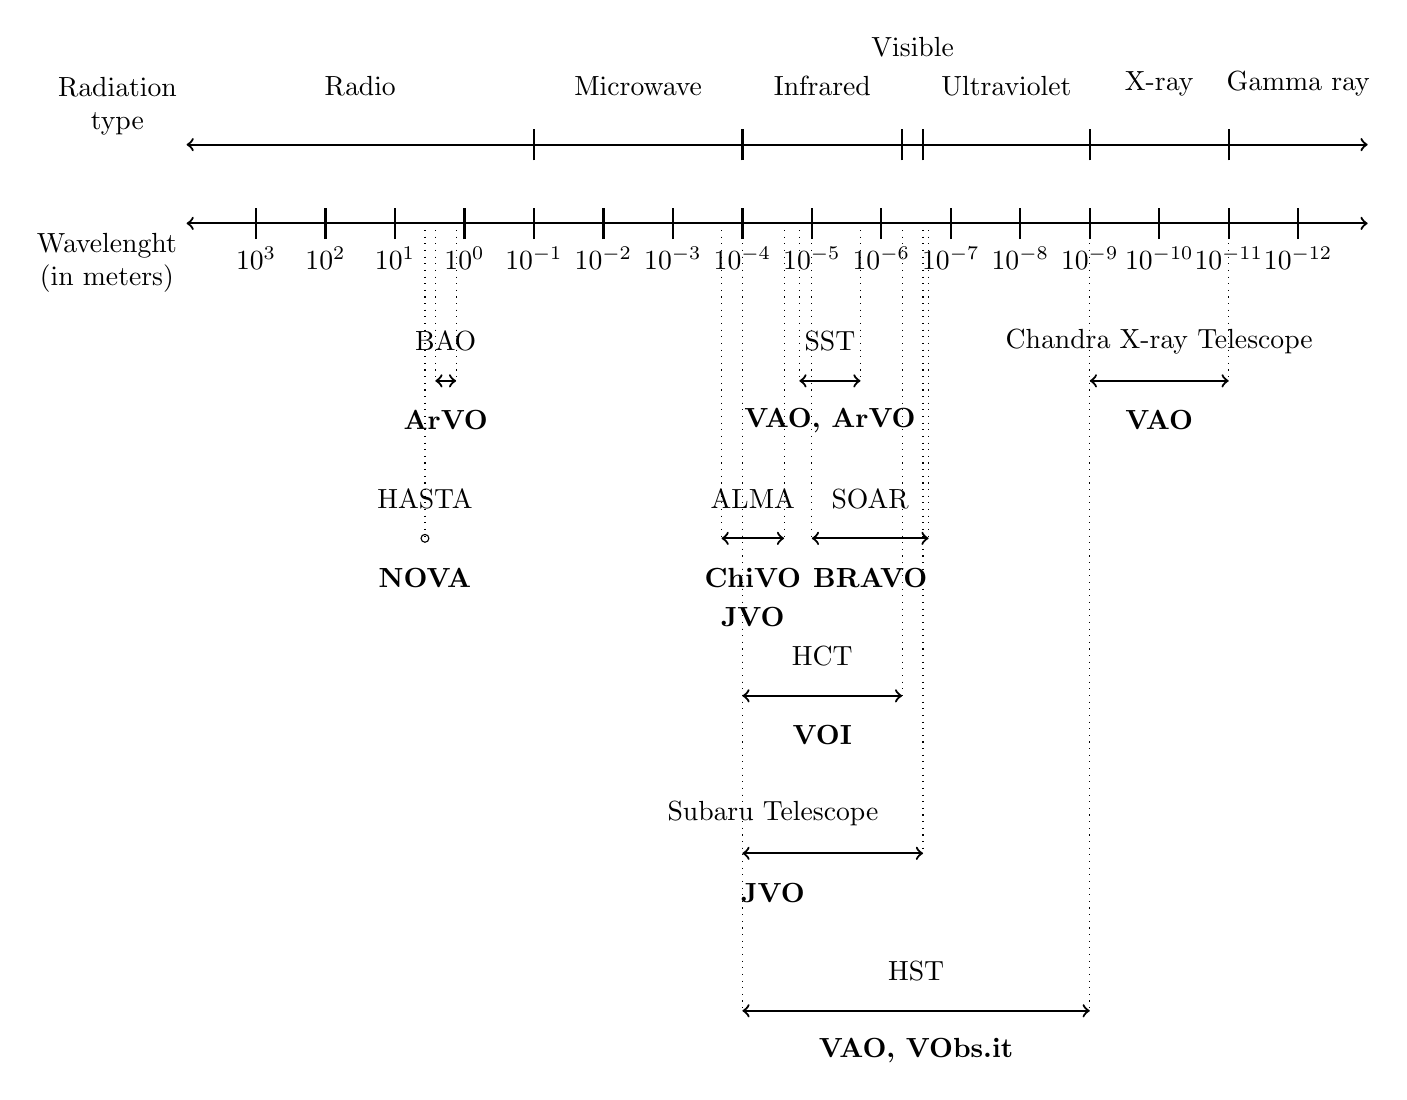
\begin{tikzpicture}
\pgfmathsetmacro{\lineLenght}{15}
\pgfmathsetmacro{\lineDivNum}{17}
\pgfmathsetmacro{\markPlace}{\lineLenght/\lineDivNum}
\def\limitsList{5,8,10.3,10.6,13,15}
\def\regionArray{{2.5,(5+8)/2,(8+10.3)/2,(10.3+10.6)/2,(10.6+13)/2,(13+15)/2,
                  (15+17)/2}}
\foreach \x in {0,1} {
  \draw[<->,thick] (0,\x) -- (\lineLenght,\x);
}
\foreach \x in \limitsList {
  \draw[thick] (\x*\markPlace,0.8) -- (\x*\markPlace,1.2);
}
\foreach \x in {1,2,...,16} {
  \pgfmathtruncatemacro{\b}{\x-2*\x+4} 
  \draw[thick] (\x*\markPlace,-0.2) -- (\x*\markPlace,0.2)
  node[pos=-0.6]{$10^{\b}$};
}
\node [anchor=north east,align=center] at (0,0) {Wavelenght\\(in meters)};
\node [anchor=south east,align=center] at (0,1) {Radiation\\type};
\node [above] at (\regionArray[0]*\markPlace,1.5) {Radio};
\node [above] at (\regionArray[1]*\markPlace,1.5) {Microwave};
\node [above] at (\regionArray[2]*\markPlace,1.5) {Infrared};
\node [above] at (\regionArray[3]*\markPlace,2) {Visible};
\node [above] at (\regionArray[4]*\markPlace,1.5) {Ultraviolet};
\node [above] at (\regionArray[5]*\markPlace,1.5) {X-ray};
\node [above] at (\regionArray[6]*\markPlace,1.5) {Gamma ray};

% Spectrum value or range for each instrument where some virtual observatory
% contributes

\pgfmathsetmacro{\factor}{\markPlace/2}
% ALMA
\draw[<->,thick] (7.7*\markPlace,-4) -- (8.6*\markPlace,-4);
\pgfmathparse{multiply(8.6-7.7,\factor)}
\node at (\pgfmathresult+7.7*\markPlace,-3.5) {ALMA};
\node at (\pgfmathresult+7.7*\markPlace,-4.5) {\textbf{ChiVO}};
\node at (\pgfmathresult+7.7*\markPlace,-5.0) {\textbf{JVO}};
 BAO
\draw[<->,thick] (3.58*\markPlace,-2) -- (3.88*\markPlace,-2);
\pgfmathparse{multiply(3.88-3.58,\factor)}
\node at (\pgfmathresult+3.58*\markPlace,-1.5) {BAO};
\node at (\pgfmathresult+3.58*\markPlace,-2.5) {\textbf{ArVO}};
% Chandra X-ray Telescope 
\draw[<->,thick] (13*\markPlace,-2) -- (15*\markPlace,-2);
\pgfmathparse{multiply(15-13,\factor)}
\node at (\pgfmathresult+13*\markPlace,-1.5) {Chandra X-ray Telescope};
\node at (\pgfmathresult+13*\markPlace,-2.5) {\textbf{VAO}};
% HASTA 
\node at (3.4312*\markPlace,-4) [inner sep=1pt,circle,draw] {};
\node at (3.4312*\markPlace,-3.5) {HASTA};
\node at (3.4312*\markPlace,-4.5) {\textbf{NOVA}};
% HCT
\draw[<->,thick] (8*\markPlace,-6) -- (10.3*\markPlace,-6);
\pgfmathparse{multiply(10.3-8,\factor)}
\node at (\pgfmathresult+8*\markPlace,-5.5) {HCT};
\node at (\pgfmathresult+8*\markPlace,-6.5) {\textbf{VOI}};
% HST  
\draw[<->,thick] (8*\markPlace,-10) -- (13*\markPlace,-10);
\pgfmathparse{multiply(13-8,\factor)}
\node at (\pgfmathresult+8*\markPlace,-9.5) {HST};
\node at (\pgfmathresult+8*\markPlace,-10.5) {\textbf{VAO, VObs.it}};
% SOAR 
\draw[<->,thick] (9*\markPlace,-4) -- (10.68*\markPlace,-4);
\pgfmathparse{multiply(10.68-9,\factor)}
\node at (\pgfmathresult+9*\markPlace,-3.5) {SOAR};
\node at (\pgfmathresult+9*\markPlace,-4.5) {\textbf{BRAVO}};
% SST
\draw[<->,thick] (8.82*\markPlace,-2) -- (9.7*\markPlace,-2);
\pgfmathparse{multiply(9.7-8.82,\factor)}
\node at (\pgfmathresult+8.82*\markPlace,-1.5) {SST};
\node at (\pgfmathresult+8.82*\markPlace,-2.5) {\textbf{VAO, ArVO}};
% Subaru Telescope
\draw[<->,thick] (8*\markPlace,-8) -- (10.6*\markPlace,-8);
\node at (\pgfmathresult+8*\markPlace,-7.5) {Subaru Telescope};
\node at (\pgfmathresult+8*\markPlace,-8.5) {\textbf{JVO}};

% Perpendicular long dotted lines

\def\firstLinesEnds{3.58,3.88,8.82,9.7,13,15}
\foreach \x in \firstLinesEnds {
  \draw[dotted] (\x*\markPlace,0) -- (\x*\markPlace,-2);
}
\def\secondLinesEnds{3.4312,7.7,8.6,9,10.68}
\foreach \x in \secondLinesEnds {
  \draw[dotted] (\x*\markPlace,0) -- (\x*\markPlace,-4);
}
\draw[dotted] (8*\markPlace,0) -- (8*\markPlace,-6);
\draw[dotted] (10.3*\markPlace,0) -- (10.3*\markPlace,-6);
\draw[dotted] (8*\markPlace,0) -- (8*\markPlace,-8);
\draw[dotted] (10.6*\markPlace,0) -- (10.6*\markPlace,-8);
\draw[dotted] (8*\markPlace,0) -- (8*\markPlace,-10);
\draw[dotted] (13*\markPlace,0) -- (13*\markPlace,-10);
\end{tikzpicture}
\caption{Virtual observatories that contributes to specifics astronomical
instruments.}
\end{center}
\label{figure:wavelength}
\end{figure}
\end{landscape}

In Figure \ref{figure:wavelength}, the different types of
radiation (in order) with their common names are shown. Below, the value of
the wavelengths in meters and the respective telescope/instrument are presented. 

%A higher $ \lambda $
%value is related with a lower frequency and a
%lower $ \lambda $ is related with a higher frequency. 
%The electromagnetic
%spectrum value or range for each instrument (above) and virtual observatory
%(below) is represented with a dot or line, respectively.\\

%\scriptsize
%\begin{table*}[h!t]
%\centering
%\begin{tabular}{|p{1cm}|p{4cm}|p{5cm}|p{6cm}|}
%    \hline                                                                      
%    \textbf{VO} & \textbf{Instrument} & \textbf{Location} &
%    \textbf{Spectrum value or range} \\
%    \hline                                                                      
%    BRAVO & Southern Astrophysical Research
%    Telescope (SOAR) & Cerro Pach\'{o}n, Chile & blue (320 nm) to near infrared
%    \cite{website:SOAR_EMS} \\
%    \hline                                                                      
%    NOVA & H-Alpha Solar Telescope for
%    Argentina (HASTA) & Leoncito, San Juan, Argentina & H-Alpha (656.28 nm)
%    \cite{website:HASTA_EMS} \\
%    \hline
%    ChiVO & Atacama Large Milimeter/submilimeter
%    Array (ALMA) & Llano de Chajnantor Observatory, Atacama Desert, Chile &
%    initially in 400 $ \mu $m to 3 mm \cite{website:ALMA_EMS} \\
%    \hline
%    \multirow{3}{3cm}{VAO} & Hubble Space
%    Telescope (HST) & 569 km above the surface of Earth & near-ultraviolet,
%    visible and near-infrared light with WFC3; ultraviolet light with COS;
%    visible light with ACS; ultraviolet, visible and near-infrared light with
%    STIS; infrared light with NICMOS \cite{website:HST_EMS} \\
%     \cline{2-4}
%     & Chandra X-ray Observatory & 139,000 km above the surface of Earth & X-ray
%     \cite{website:Chandra_EMS} \\
%     \cline{2-4}
%     & Spitzer Space Telescope (SST) & 176,602,814 km above the surface of Earth
%     \cite{website:SST_EMS_1} & 3 $ \mu $m to 180 $ \mu $m
%     \cite{website:SST_EMS_2} \\
%    \hline
%    ArVO & Byurakan Astrophysical Observatory
%    (BAO) & Mount Aragats, Armenia & 1.2 m and 4.2 m \cite{website:BAO_EMS} \\
%    \hline
%    ArVO & Spitzer Space Telescope (SST) &
%    176,602,814 km above the surface of Earth & 3 $ \mu $m to 180 $ \mu $m \\
%    \hline
%    Vobs.it & Hubble Space Telescope (HST) & 569
%    km above the surface of Earth & near-ultraviolet, visible and near-infrared
%    light with WFC3; ultraviolet light with COS; visible light with ACS;
%    ultraviolet, visible and near-infrared light with STIS; infrared light with
%    NICMOS \\
%    \hline
%    \multirow{2}{3cm}{UkrVO} & Main Astronomical
%    Observatory (MAO) & Kiev, Ukraine & \\
%     \cline{2-4}
%     & Mykolaiv Astronomical Observatory & Mykolaiv, Ukraine & \\
%    \hline
%    \multirow{3}{3cm}{JVO} & Subaru Telescope &
%    Mauna Kea, Big Island, Hawaii & visible and infrared light
%    \cite{website:Subaru_EMS} \\
%     \cline{2-4}
%     & Sloan Digital Sky Survey (SDSS) & Sacramento Mountains, Sunspot, New
%     Mexico, USA & \\
%     \cline{2-4} 
%     & Atacama Large Milimeter/submilimeter Array (ALMA) & Llano de Chajnantor
%     Observatory, Atacama Desert, Chile & initially in 400 $ \mu $m to 3 mm \\
%    \hline
%    VOI & Himalayan Chandra Telescope (HCT) & Mount
%    Saraswati, Digpa-ratsa Ri, Hanle, India & infrared light 
%    \cite{website:HCT_EMS} \\
%    \hline
% \end{tabular}
%\caption{Virtual observatories that contributes to specifics astronomical
%instruments.}
%\label{table:vo_EMS}
%\end{table*}
%%\end{longtable}
%%\end{center}
%\normalsize



\section{Conclusions and Recommendations}
At present the distribution of the virtual observatories in the world is not
related with the astronomical installations, i.e., only ESO (European Souther
Observatory) operates in three places in the north of Chile: La Silla, Paranal
and
Chajnantor\footnote{\url{http://www.eso.org/public/chile/about-eso/cooperation.html}},
but there still does not exist the presence of the Virtual Observatory (VO).
The 47\% of virtual observatories have been founded by the members of European
Community.\\

The membership of the International Virtual Observatory Alliance does not imply
the constant contribution from the astronomy activity, this is independent,
because the IVOA is a initiative which intends to share the astronomical
knowledge between them and the community in a standardized manner.  On the
other hand, during the research, was visualized that have not been updated the
status projects of some virtual observatories from the official sources or the
data is not accesible from a web platform.\\

The development and implementing of a virtual observatory in Chile is urgent.
Chile is an astronomer's
paradise\footnote{\url{http://www.bbc.co.uk/news/world-latin-america-14205720}}.
A platform under the IVOA's standards from there allows to facilitate the
Chileans and global astronomical contributions, among others.\\

Countless of tools could be developed from a Chilean virtual observatory. These
applications would respond to the currents and future needs for any member of
IVOA. The International Virtual Observatory Alliance has the Working Groups
which works to development the standards that would later all members will be
submitted.\\


\section*{Acknowledges}
This research was possible due to CONICYT-Chile fundings, specifically 
through the project FONDEF D11I1060 and the project ICHAA 79130008.
\section{References}

\bibliographystyle{plain}
\bibliography{ac2014.bib}

%\appendix

%\subsection{Summary of Tools and Projects}

The standards and services of a VO are meant to be used in the end 
by applications. The Applications working group have defined only two major
standards for application interoperability beyond the services standards: 
(1) the Simple Application Messaging Protocol (SAMP), and (2) the VOTable
format. These standards, plus all the other protocols and standards 
allows VO-compliant tools to be developed, which are the endpoints for
science production. In the next table we summarize the most used tools
and they status.

%%%%%%%%%%%%%%%%%%%%%%%%%%%%%%%%%%%%%%%%%%%%%%%%%%%%%%%%%%%%%%%%%%%%%%%%%%%%%%%%%
%%%%%%%%%%%%%%%%%%%%%%%%%%%%%%%%%$Data Access%%%%%%%%%%%%%%%%%%%%%%%%%%%%%%%%%%%%
%%%%%%%%%%%%%%%%%%%%%%%%%%%%%%%%%%%%%%%%%%%%%%%%%%%%%%%%%%%%%%%%%%%%%%%%%%%%%%%%%
\begin{table*}[h]
	\centering
	\begin{tabular}{|l|l|p{8.5cm}|}
	\hline
	\textbf{User Tool} & \textbf{Country} &  \textbf{Comment}\\
	\hline
  Cross-Comparision Tool & USA & a web tool that performs croos-comparisons between one table supplied by the user and other of an online source 
								catalog, for a user-specified match radius. This returns the all sources in the online catalog that are within the radius.\\
	\hline								 
  Data Discovery Tool & USA &  A web tool that allows to find datasets from astronomical collections known to the VO like the Hubble Space Telescope 
									(HST), the Chandra X-ray Observatory, the Spitzer Space Telescope, among other.\\
	\hline								 
  Time Series Search Tool & USA & A web tool that allows to access the time series data sets at the Harvard Time Series Center (TSC), the NASA 
									Exoplanet Archive and the Catalina Real-Time Transient Survey, and analize them with the periodogram application 
									of the NASA Exoplanet Archive.\\
  \hline
  Iris & USA & A downloadable application for the finding, plotting and fitting the 
			Spectral Energies Distributions (SEDs). \\
	\hline								 
  Seleste & USA & \\
	\hline								 
  Skyview & USA & \\
	\hline								 
  Specview & USA & \\
  \hline
  WCSFIXER & USA & \\
  \hline 
  Montage & USA & \\
  \hline
  Xamin & USA & \\
	\hline								 
  Aladin & France & Widely-used VO tool that allows searching, visualizing
and perform basic operation to images, spectra and catalogs.\\
	\hline								 
  Cassis & France & \\
	\hline								 
  Cross-Match Service & France  & \\
	\hline								 
  AppLauncher & France & \\
	\hline								 
  X-Match & France & \\
	\hline								 
   VOSA & Spain & \\
	\hline								 
  VOSED & Spain & \\
	\hline								 
  TESELA & Spain &  a service that allows to access the catalog of blank
regions. It is based on the application of the Delaunay triangulation\\
	\hline								 
  Filter Profiles & Spain & \\
   \hline
	VODesktop & UK & an analysis tools wich allows limit the choice of resources through specific data saving.\\
	\hline								 
  Topcat & UK &  An interactive graphical viewer and editor for tabular data for
formats like the Flexible Image Transport System (FITS) \\
	\hline								 
	\hline								 
  Splat & Germany & \\
	\hline								 
   VOSpec & Europe & A multi-wavelength spectral analysis tool with access to
atomic and \\
	\hline								 
 AstroStat & India & a software tool that allows astronomers to use both and sophisticated statical routines on large datasets uploaded in VOTable or
									ASCII format. \\
	\hline								 
  Visivo & Italy & \\
	\hline								 
	Skynode & Italy & A web service that allows to query in the VVDS catalogs. \\
	\hline		
	\end{tabular}
	\caption{Data Access}
	\label{table:da}
\end{table*}





% that's all folks
\end{document}


